\subsection{Aproximación cuasiestática}
Los campos electromagnéticos presentan diferentes propiedades propiedades según la región en la que se encuentren. Al considerar las dimensiones de la fuente  del orden $d$ y la longitud de onda $\lambda=2\pi c/\omega$, entonces hay tres regiones de interés: la región cercana (estática) en donde $d\ll r\ll\lambda$, que se estudiará en la siguiente sección, la región intermedia en donde $d\ll r\sim \lambda$, y la región lejana (de radiación) donde $d\ll \lambda\ll r$ \cite{Jackson}.
\subsubsection{Dipolo eléctrico (caso estático)}

En electrodinámica clásica, se entiende como \textit{límite cuasiestático} el considerar una partícula de tamaño mucho menor que la longitud de onda de la luz incidente \cite{Cuasiest}. En el caso de un elipsoide caracterizado por una función dieléctrica $\epsilon_p$, que se encuentra inmerso en un medio caracterizado por una función dieléctrica $\epsilon_m$ y cuyo semieje mayor es $a$, se puede definir el límite cuasiestático cuando el parámetro de tamaño $x=ka$ es mucho menor que la unidad \cite{Bohren}, donde $k=2\pi \sqrt{\epsilon_m}/\lambda$. Esta aproximación garantiza que toda la geometría del elipsoide esté sujeta a un campo eléctrico de la misma intensidad y dirección \cite{Miguel}.\\


En la aproximación cuasiestática, es posible analizar a la partícula mediante la aproximación dipolar, al considerar a las cargas que conforman un dipolo eléctrico embebidas en un medio homogéneo e infinito caracterizado por su función dieléctrica $\epsilon_m$. Con esta aproximación, se obtiene el potencial eléctrico para un dipolo puntual \cite{Griffiths}:
\begin{equation}
\phi=\frac{p}{4\pi\epsilon_m}\left(\frac{\Vec{r}\cdot\hat{e}_z}{r^3}\right)=\frac{\Vec{p}\cdot\Vec{r}}{4\pi\epsilon_m r^3}=\frac{p\cos\theta}{4\pi\epsilon_m r^2}
\label{pot_dipolo}
\end{equation}
donde $\Vec{p}$ representa el momento dipolar eléctrico. Si se considera una esfera con permitividad eléctrica $\epsilon_p$, embebida en el mismo medio caracterizado por su función dieléctrica $\epsilon_m$ en el cual existe un campo eléctrico uniforme $\Vec{E}_0=E_0\hat{e}_z$, al resolver la ecuación de Laplace considerando las condiciones de frontera entre la esfera y el medio, se obtiene que el campo eléctrico fuera de la esfera es la superposición del campo eléctrico aplicado y del campo eléctrico producido por un dipolo eléctrico puntual localizado en el origen con momento dipolar \cite{Bohren}:
\begin{equation}
	\vec{p}= \epsilon_m\alpha\Vec{E}_0=4\pi\epsilon_m a^3\frac{\epsilon_1-\epsilon_m}{\epsilon_1+2\epsilon_m}\Vec{E}_0,
	\label{momentdipol}
\end{equation}
donde $\alpha=4\pi a^3(\epsilon_1-\epsilon_m)/(\epsilon_1+2\epsilon_m)$ es la polarizabilidad eléctrica, que representa la facilidad con la que se polariza la esfera. Es decir, el campo eléctrico induce un dipolo eléctrico en la esfera.
\begin{figure}[h!]
	\includegraphics[width=6cm]{../../Figuras/shereE0}
	\caption{Esfera de radio $r$ caracterizada por su función dieléctrica $\epsilon_p$ y embebida en un medio caracterizado por su función dieléctrica $\epsilon_$ en la cual incide un campo eléctrico uniforme $\Vec{E}_0$.}
\end{figure}


\subsubsection{Dipolo eléctrico (caso dinámico)}}

El potencial de la sección anterior considera que las cargas se encuentran fijas en el espacio y están sometidas a un campo eléctrico homogéneo. Este potencial correspondería al de una partícula elipsoidal con una polarización $\Vec{p}$ a determinar, en presencia de un campo eléctrico homogéneo alineado en la dirección $\hat{e}_z$. El siguiente escenario a considerar es de las cargas localizadas en un volumen finito moviéndose en presencia de un campo eléctrico dinámico. Una forma de solucionar este problema es considerar que el movimiento de los campos, y por lo tanto de las cargas y corrientes, es armónico; lo cual es equivalente a realizar un análisis en componentes de Fourier. De esta forma, no se pierde generalidad de considerar a los potenciales y campos de un sistema de cargas y corrientes localizadas en el espacio vacío, con una dependencia armónica variando en el tiempo y que oscilan a la frecuencia $\omega$ del campo electromagnético aplicado \cite{Jackson}
\begin{align}
    \rho(\Vec{r},t)&=\rho(\Vec{r})e^{-i\omega t},\nonumber\\
    \Vec{J}(\Vec{r},t)&=\Vec{J}(\Vec{r})e^{-i\omega t},
    \label{armonicf}
\end{align}
considerando que el significado físico lo posee la parte real. Mediante lo anterior, es posible determinar los campos electromagnéticos mediante el potencial vectorial como \cite{Jackson}:
\begin{align*}
  \Vec{A}(\Vec{r},t)=\frac{\mu_0}{4\pi}\int \text{d}^3r'\frac{\Vec{J}(\Vec{r'})e^{i\omega \frac{|\Vec{r}-\Vec{r'}|}{c}}}{|\Vec{r}-\Vec{r'}|}e^{-i\omega t},
\end{align*}
en donde se emplea la norma de Lorentz \cite{Griffiths} y la densidad de corriente se evalúa en el tiempo de retardo $t_r=t-|\Vec{r}-\Vec{r'}|/c$. Al definir $k=\omega/c$ y obviando la dependencia temporal
\begin{equation}
    \Vec{A}(\Vec{r},t)=\frac{\mu_0}{4\pi}\int \Vec{J}(\Vec{r'})\frac{e^{ik|\Vec{r}-\Vec{r'}|}}{|\Vec{r}-\Vec{r'}|} \text{d}^3r'.
    \label{pot_vectorial}
\end{equation} 

En la región de campo cercano, donde $r\ll\lambda$ (o $kr\ll 1$),  exp($ik|\Vec{r}-\Vec{r'}|)\to 1$, se tiene \cite{Jackson}
\begin{equation*}
	\Vec{A}(\Vec{r},t)=\frac{\mu_0}{4\pi}\int \frac{\Vec{J}(\Vec{r'})}{|\Vec{r}-\Vec{r'}|} \text{d}^3r',
\end{equation*} 
mientras que en la región de campo lejano ($kr\gg 1$) dado que la exponencial oscila rápidamente, es suficiente aproximar
\begin{equation}
	|\Vec{r}-\Vec{r'}|\simeq r-\hat{e}_r\cdot\Vec{r'},    
\end{equation}
con $\hat{e}_r$ un vector unitario en la dirección de $\Vec{r}$. \footnote{Empleando la ley de cosenos y haciendo una expansión binomial $
	|\Vec{r}-\Vec{r'}|=\sqrt{r^2+(r')^2-2rr'\cos\theta}=r\sqrt{1+\left(r'/r\right)^2-2\left((r'/r)\cos\theta\right)}\simeq r\left\{1-(\hat{e}_r\cdot\Vec{r'}/r)+1/2\left(r'/r\right)^2\right\}\simeq r-\hat{e}_r\cdot\Vec{r'}.$} Si sólo se consideran los términos que decaen como $r^{-1}$, el inverso de la distancia en la Ec. (\ref{pot_vectorial}) puede ser reemplazado por $r$. Entonces, el potencial vectorial es
	\begin{equation*}
	\lim_{kr\rightarrow\infty}\Vec{A}(\Vec{r})=\frac{\mu_0}{4\pi}\frac{e^{ikr}}{r}\int \Vec{J}(\Vec{r'})e^{-ik\hat{e}_r\cdot\Vec{r'}}\text{d}^3r',    
	\end{equation*}
	que se puede reescribir al realizar la expansión en serie de potencias de la exponencial dentro de la integral de volumen, dando como resultado
	\begin{equation*}
	\lim_{kr\rightarrow\infty}\Vec{A}(\Vec{r})=\frac{\mu_0}{4\pi}\frac{e^{ikr}}{r}\sum_n\frac{(-ik)^n}{n!}\int \Vec{J}(\Vec{r'})(\hat{e}_r\cdot\Vec{r'})^n \text{d}^3r'.    
	\end{equation*}
\begin{figure}[h!]
	\includegraphics[width=6cm]{../../Figuras/aprox.jpg}
	\caption{Vector de posición $\Vec{r}$ del volumen y $\Vec{r'}$. Se muestra la distancia $|\Vec{r}-\Vec{r'}|$ entre estos últimos. }
\end{figure}
Al considerar únicamente el primer término de la expansión, se concluye que 
\begin{equation}
    \Vec{A}(\Vec{r})\approx\frac{\mu_0}{4\pi}\frac{e^{ikr}}{r}\int \Vec{J}(\Vec{r'}) \text{d}^3r',    
    \label{aprox_pot_vec}
\end{equation}
que al realizar una integración por partes,  \footnote{Al considerar $\int_V \Vec{r'}(\nabla'\cdot\Vec{J})\text{d}^3r'=\int_{\partial V} \Vec{r'}(\Vec{J}\cdot \text{d}\Vec{S})-\int_V \Vec{J}\text{d}^3r'$ y asumiendo que $\Vec{J}$ se desvanece en los límites del volumen $V$, es decir, en la superficie $\partial V$. } se obtiene que
\begin{equation}
	\int\Vec{J}d^3r'=-\int \Vec{r'}(\nabla'\cdot\Vec{J})\text{d}^3r'=-i\omega\int \Vec{r'}\rho(\Vec{r'})\text{d}^3r',
	\label{Jrho}
\end{equation}
donde se emplea
\begin{equation*}
    \nabla\cdot\Vec{J}=-\frac{\partial\rho}{\partial t}=i\omega\rho(\Vec{r}). 
\end{equation*}
Al sustituir la Ec. (\ref{Jrho}) en la Ec. (\ref{aprox_pot_vec}) y considerando que el momento dipolar eléctrico $\Vec{p}$ de una distribución de cargas $\rho$ es
\begin{equation*}
	\Vec{p}=\int \Vec{r'}\rho(\Vec{r'})\text{d}^3r',
\end{equation*}
se obtiene 
\begin{equation}
    \Vec{A}(\Vec{r})=-\frac{i\omega\mu_0}{4\pi}\frac{e^{ikr}}{r}\int \Vec{r'}\rho(\Vec{r'})\text{d}^3r'=-\frac{i\omega\mu_0}{4\pi}\frac{e^{ikr}}{r}\Vec{p}. 
    \label{A_dip}  
\end{equation}
Al calcular el campo $\Vec{H}$ como función del potencial vectorial, y empleando la ley de Faraday-Lenz para determinar el campo eléctrico, se concluye que \cite{Jackson}
\begin{align}
	\Vec{E}&=\frac{1}{4\pi\epsilon_0}\left\{k^2(\hat{e}_r\times\Vec{p})\times\hat{e}_r\frac{e^{ikr}}{r}+[3\hat{e}_r(\hat{e}_r\cdot\Vec{p})-\Vec{p}]\left(\frac{1}{r^3}-\frac{ik}{r^2}\right)e^{ikr}\right\},\\
    \Vec{H}&=\frac{ck^2}{4\pi}(\hat{e}_r\times\Vec{p})\frac{e^{ikr}}{r}\left(1-\frac{1}{ikr}\right).    
\end{align}
Obsérvese que el campo $\Vec{H}$ es transversal al vector radial para cualquier distancia, mientras el campo eléctrico tiene componentes paralelas y perpendiculares a $\hat{e}_r$.\\ 

\noindent Con base en la Ec. (\ref{A_dip}), en la zona de radiación cuando $kr\gg 1$, se tiene que al iluminar el sistema con una onda plana armónica en el tiempo y de frecuencia angular $\omega$ se induce un dipolo eléctrico $p$ que genera campos electromagnéticos $\Vec{E}_p$ y $\Vec{H}_p$ que oscilan a la misma frecuencia $\omega$ 
\begin{align}
    \Vec{E}_p&=\frac{e^{ikr}}{-ikr}\frac{ik^3}{4\pi\epsilon_m}\hat{e}_r\times(\hat{e}_r\times \Vec{p}) e^{i\omega t}, \hspace{1cm}
    \Vec{H}_p=\frac{ck^2}{4\pi}(\hat{e}_r\times\Vec{p})\frac{e^{ikr}}{r}e^{i\omega t}.
\end{align}
Si de manera similar a la Ec. (\ref{momentdipol}), se considera un campo eléctrico oscilante polarizado en la dirección $\hat{e}_x$, que induce un dipolo eléctrico con momento dipolar  $\Vec{p}=\epsilon_m \alpha E_0 e^{-i\omega t}\hat{e}_x$, se pueden reescribir a los campos generados por el dipolo inducido mediante el vector de amplitud de esparcimiento
\begin{equation}
	\Vec{X}=\frac{ik^3}{4\pi}\alpha \hat{e}_r\times(\hat{e}_r\times \hat{e}_x),
	\label{Xvec}
\end{equation}
como
 \begin{align}
 	\Vec{E}_{p}&=\frac{e^{ik(r-z)}}{-ikr}\Vec{X}E,
 	\hspace{1cm}
 	\Vec{H}_{p}=\frac{k}{\omega\mu}\hat{e}_r\times\Vec{E}_{s}.
 	\label{EH_s}
 \end{align}
donde $E=E_0 e^{ikz}$ y la polarización en la base de vectores esféricos es $\Vec{p}=\epsilon_m \alpha E_0 e^{-i\omega t}(\sin\theta\cos\phi\: \hat{e}_r+\cos\theta\cos\phi\: \hat{e}_{\theta}-\sin\phi \:\hat{e}_{\phi})$. \footnote{Es decir, $\hat{e}_r\times(\hat{e}_r\times \hat{e}_x)=-\cos\theta\cos\phi \hat{e}_{\theta}+\sin\phi \hat{e}_{\phi}$. } \\

